\documentclass{standalone}

\usepackage{tikz}

\newcounter{num}
\newcommand{\tictactoe}[1]
    {\begin{tikzpicture}[line width=1pt, scale=0.5]
            \def\r{0.125}
            \tikzset{
                circ/.pic={\draw circle (\r);},
                cross/.pic={\draw (-\r,-\r) -- (\r,\r) (-\r,\r) -- (\r,-\r);},
                opt/.pic={\draw[opacity=0.2] (-\r,-\r) -- (\r,\r) (-\r,\r) -- (\r,-\r);}
            }
            % The grid
            \foreach \i in {1,2} \draw (\i,0) -- (\i,3) (0,\i) -- (3,\i);
            % Numbering the cells
            \setcounter{num}{0}
            \foreach \y in {0,...,2}
            \foreach \x in {0,...,2} {
                    \coordinate (\thenum) at (\x+0.5,2-\y+0.5);
                    %\node[opacity=0.5] at (\thenum) {\sffamily\thenum}; % Uncomment to see numbers in the cells
                    \addtocounter{num}{1}
                }
            \def\X{X} \def\x{x} \def\O{O} \def\n{n}
            \foreach \l [count = \i from 0] in {#1} {
                    \if\l\X \path (\i) pic{cross};
                    \else
                        \if\l\O \path (\i) pic{circ};
                        \else
                            \if\l\x \path (\i) pic{opt};
                            \else
                                \if\l\n \node[opacity=0.5] at (\i) {\sffamily\i};
                                \fi
                            \fi
                        \fi
                    \fi
                }
        \end{tikzpicture}}

\begin{document}
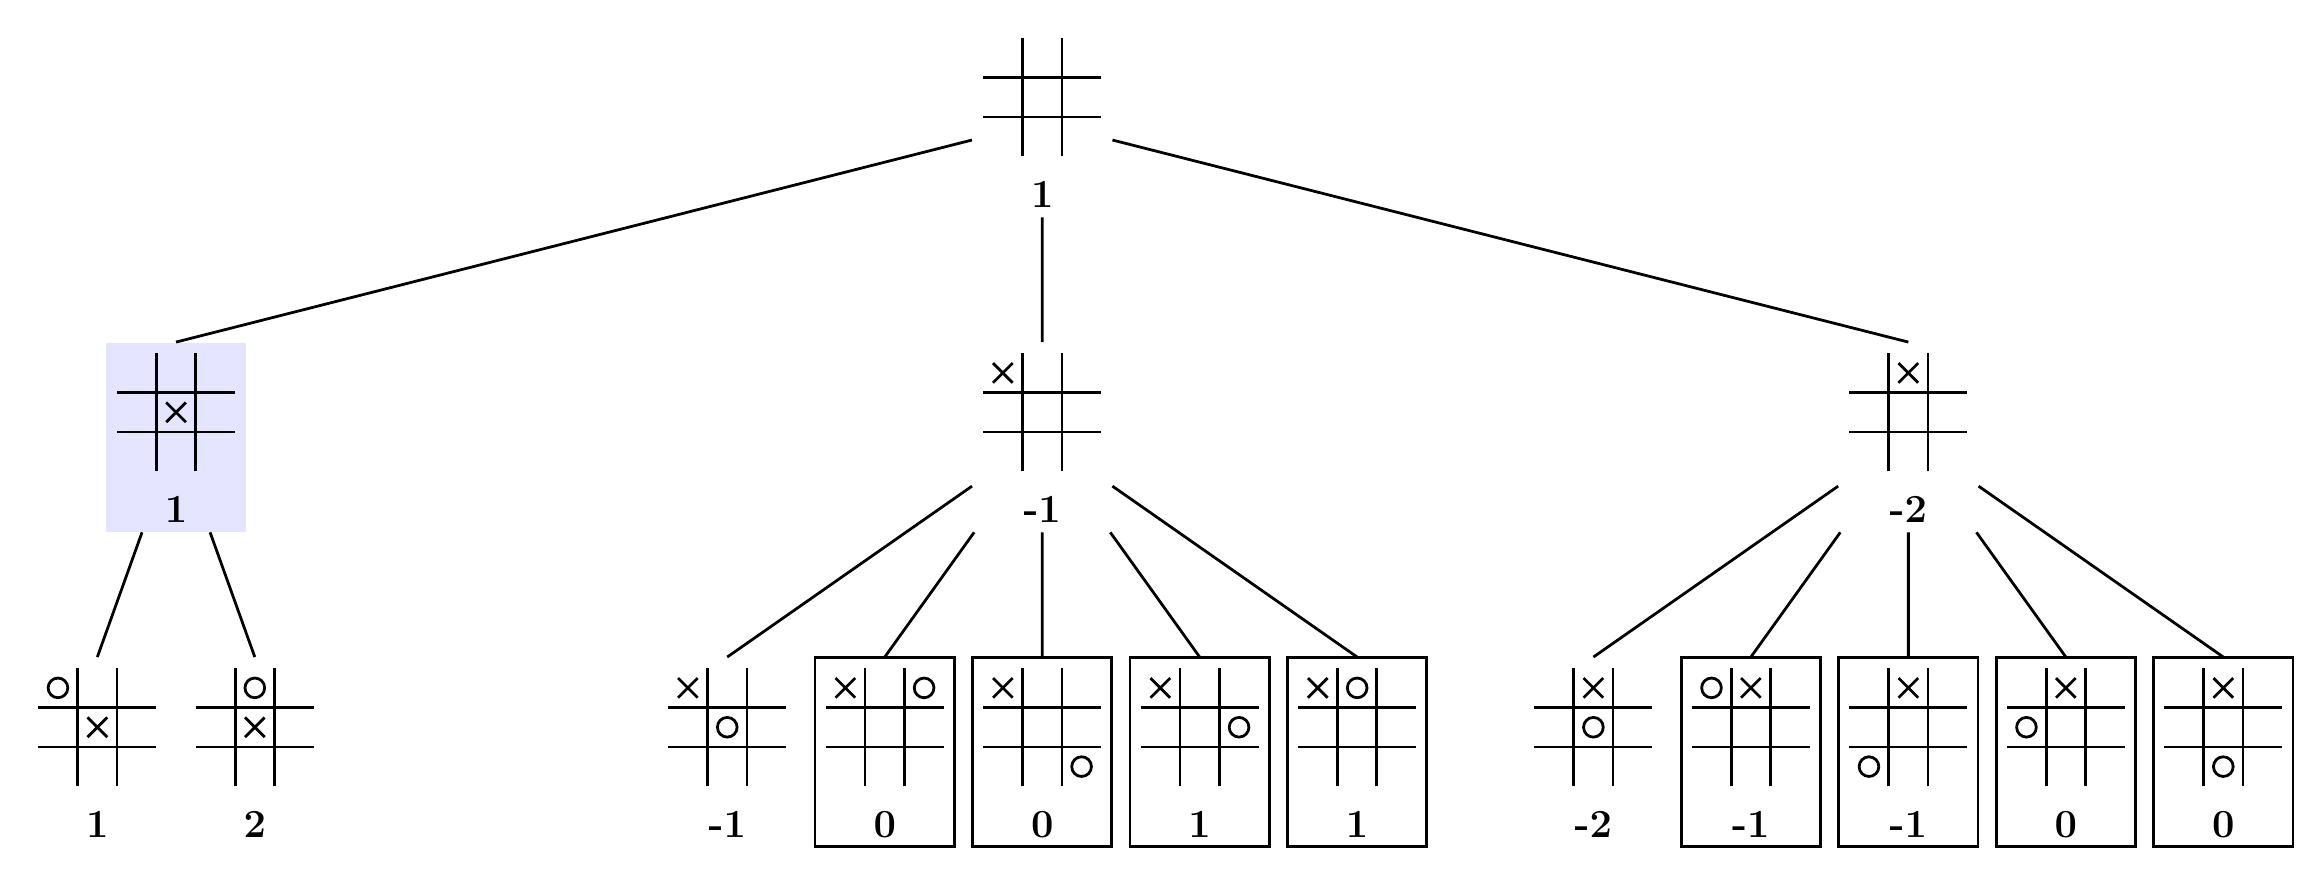
\begin{tikzpicture}[
        line width=1pt,
        child anchor=north,
        every node/.style={auto, align=center, text centered, font=\Large\bfseries, },
        optimal/.style={fill=blue!10},
        cut/.style={rectangle, draw},
        level/.style={level distance=4cm},
        level 1/.style={sibling distance=11cm},
        level 2/.style={sibling distance=2cm},
    ]
    \node {
        \tictactoe{
            , , ,
            , , ,
            , , ,
        } \\
        1
    }
    child {
            node[optimal] {
                    \tictactoe{
                        , , ,
                        , X, ,
                        , , ,
                    } \\
                    1
                }
            child {
                    node {
                            \tictactoe{
                                O, , ,
                                , X, ,
                                , , ,
                            } \\
                            1
                        }
                }
            child {
                    node {
                            \tictactoe{
                                , O, ,
                                , X, ,
                                , , ,
                            } \\
                            2
                        }
                }
        }
    child {
            node {
                    \tictactoe{
                        X, , ,
                        , , ,
                        , , ,
                    } \\
                    -1
                }
            child {
                    node {
                            \tictactoe{
                                X, , ,
                                , O, ,
                                , , ,
                            } \\
                            -1
                        }
                }
            child {
                    node[cut] {
                            \tictactoe{
                                X, , O,
                                , , ,
                                , , ,
                            } \\
                            0
                        }
                }
            child {
                    node[cut] {
                            \tictactoe{
                                X, , ,
                                , , ,
                                , , O,
                            } \\
                            0
                        }
                }
            child {
                    node[cut] {
                            \tictactoe{
                                X, , ,
                                , , O,
                                , , ,
                            } \\
                            1
                        }
                }
            child {
                    node[cut] {
                            \tictactoe{
                                X, O, ,
                                , , ,
                                , , ,
                            } \\
                            1
                        }
                }
        }
    child {
            node {
                    \tictactoe{
                        , X, ,
                        , , ,
                        , , ,
                    } \\
                    -2
                }
            child {
                    node {
                            \tictactoe{
                                , X, ,
                                , O, ,
                                , , ,
                            } \\
                            -2
                        }
                }
            child {
                    node[cut] {
                            \tictactoe{
                                O, X, ,
                                , , ,
                                , , ,
                            } \\
                            -1
                        }
                }
            child {
                    node[cut] {
                            \tictactoe{
                                , X, ,
                                , , ,
                                O, , ,
                            } \\
                            -1
                        }
                }
            child {
                    node[cut] {
                            \tictactoe{
                                , X, ,
                                O, , ,
                                , , ,
                            } \\
                            0
                        }
                }
            child {
                    node[cut] {
                            \tictactoe{
                                , X, ,
                                , , ,
                                , O, ,
                            } \\
                            0
                        }
                }
        }
    ;
\end{tikzpicture}

\end{document}










































